%%%%%%%%%%%%%%%%%%%%%%%%%%%%%%%%%%%%%%%%%%%%%%%%%%%%%%%%%%%%%%%%%%
%%%%%%%% ICML 2016 EXAMPLE LATEX SUBMISSION FILE %%%%%%%%%%%%%%%%%
%%%%%%%%%%%%%%%%%%%%%%%%%%%%%%%%%%%%%%%%%%%%%%%%%%%%%%%%%%%%%%%%%%

% Use the following line _only_ if you're still using LaTeX 2.09.
%\documentstyle[icml2016,epsf,natbib]{article}
% If you rely on Latex2e packages, like most moden people use this:
\documentclass{article}

% use Times
\usepackage{times}
% For figures
\usepackage{graphicx} % more modern
%\usepackage{epsfig} % less modern
\usepackage{subfigure} 

% For citations
\usepackage{natbib}

% For algorithms
\usepackage{algorithm}
\usepackage{algorithmic}

% As of 2011, we use the hyperref package to produce hyperlinks in the
% resulting PDF.  If this breaks your system, please commend out the
% following usepackage line and replace \usepackage{icml2016} with
% \usepackage[nohyperref]{icml2016} above.
\usepackage{hyperref}
\usepackage{graphicx}
\graphicspath{ {images/} }
% Packages hyperref and algorithmic misbehave sometimes.  We can fix
% this with the following command.
\newcommand{\theHalgorithm}{\arabic{algorithm}}

% Employ the following version of the ``usepackage'' statement for
% submitting the draft version of the paper for review.  This will set
% the note in the first column to ``Under review.  Do not distribute.''
\usepackage{icml2016} 

% Employ this version of the ``usepackage'' statement after the paper has
% been accepted, when creating the final version.  This will set the
% note in the first column to ``Proceedings of the...''
%\usepackage[accepted]{icml2016}


% The \icmltitle you define below is probably too long as a header.
% Therefore, a short form for the running title is supplied here:
\icmltitlerunning{Submission and Formatting Instructions for ICML 2016}

\begin{document} 

\twocolumn[
\icmltitle{Prediction of winner in NBA basketball games}

% It is OKAY to include author information, even for blind
% submissions: the style file will automatically remove it for you
% unless you've provided the [accepted] option to the icml2016
% package.
\icmlauthor{Zejian Zhan}{zejian.zhan@vanderbilt.edu}
\icmladdress{Vanderbilt University, Nashville, TN, 37240}

% You may provide any keywords that you 
% find helpful for describing your paper; these are used to populate 
% the "keywords" metadata in the PDF but will not be shown in the document
\icmlkeywords{sports prediction, machine learning, ICML}

\vskip 0.3in
]

\begin{abstract} 
I apply three machine learning approaches: Support Vector Machine(SVM), Linear Regression, MultipleLayer Perceptron to predict the winner of a National Basketball Association(NBA) game. The data is selected from the historical statistics of regular season games and the features are defined and computed from it. The accuracy of all algorithms is beyond 64\% by the naive majority voting mechanism. And the MLP does the best job.\end{abstract} 

\section{Introduction}
\label{submission}
The National Basketball Association is the premier men's professional basketball league in the world.The winner team within the NBA will gain popularity and get more income, and is beneficial to the league and its players. So predicting the winner in a game based on the previous performance is very valuable to business managers, coaches, players, fans, gamblers, and statisticians alike. I apply approaches to improve this prediction.\\
So far some people used the statistics of the teams like the average score, the shot efficiency and so on, while some people focused on the past history of the team like the winning percentage of the team, the overall behavior in the past ten games and the points differential. I'm trying to combining the features together to take a deeper look at both the behaviors and the historical data of the team.  I've gathered the regular seasons game box scores from 2010 to 2016 and tried to compute the feature vectors. After that I'll start to get the teams' behaviors and apply PCA(Principal Component Analysis) to analyze the most important features. At last, I'll use three approaches for machine learning process and compare the result with that generated by the naive majority voting mechanism based on the winning percentage of a team.
\section{Model} 
 I'm trying to combine the detailed behaviors statistics with the comprehensive situation of teams together and then use three approaches for training and prediction. The first big problem is where to gather the data. I searched the Internet and read the paper and finally decided to fetch data from http://www.basketball-reference.com. I can also gather the detailed behaviors of teams in each game, but it'll take more time. The accuracy of this learning system mainly depends on whether your features are well defined or not. 
 Intuitively, we will consider winning percentage of both teams. Also point differential per game is a good feature to measure the strength of a team. In addition to these, we should also look at recent behaviors of both teams so we define the win percentage and point differential per game for the latest N games. Last but not least, To define the features, there're ten features to take into consideration:
\begin{itemize}
\item {Winning percentage of team A}
\item {Winning percentage of team B}
\item {Point differential per game of team A}
\item {Point differential per game of team B}
\item {Winning percentage of team A in latest N games}
\item {Winning percentage of team B in latest N games}
\item {Point differential per game of team A in latest N games}
\item {Point differential per game of team B in latest N games}
\item {As a visiting team winning percentage of team A}
\item {As a home team winning percentage of team B}
\end{itemize}

So the aim of the following job is to collect data and generate the feature vectors for the overall behaviors of both teams in a match. And then I'll implement three machine learning processes with ten features to show that the accuracy is better.
% Acknowledgements should only appear in the accepted version. 
 From the website, I can collect the box scores of regular season game from 2011-2012 to 2015-2016. What I did to extract the data was to copy the box scores into a spreadsheet in $Excel$, and then I wrote a $macro$ to replace all the team names with numbers ranging from 1 to 30. After that, I converted .xlsx file to .txt with space splitting each instance. Note that some teams changed their name in 2013 or 2014, so I had to find it out and replace it manually. Since the data was generated in the order of ascending time. So I deleted the date and detailed time of the games and added an column for labeling whether team A was the winner or not. If so, the label is 1. Otherwise it's 0. 
 \\
 The original data was like the illustration shows:
  \begin{figure}[htbp]
 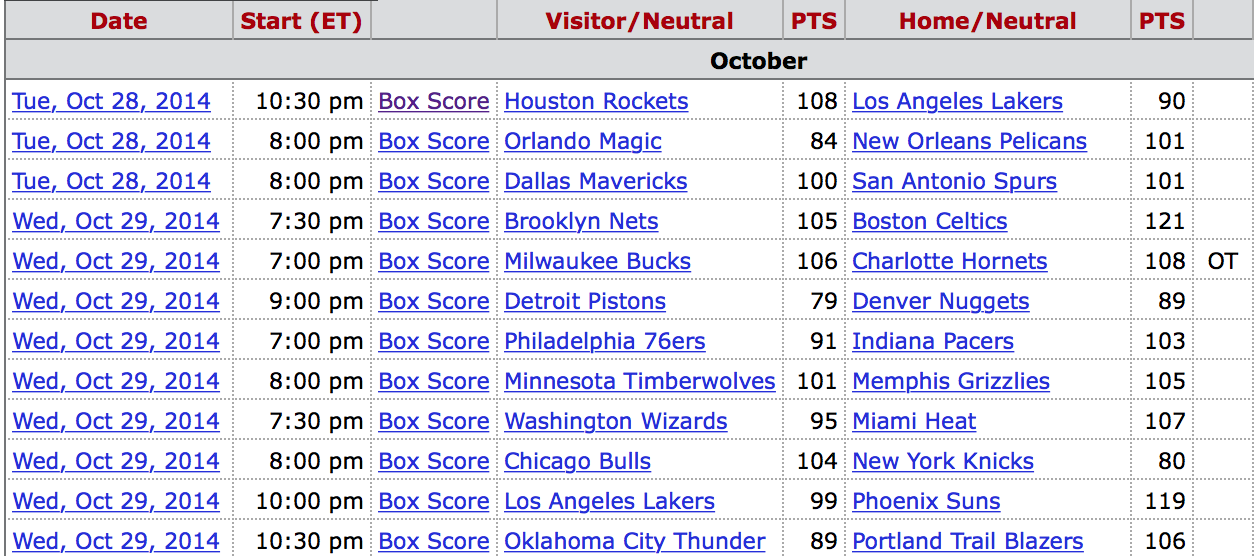
\includegraphics[width=8cm, height=4cm]{datasource}
 \caption{original data}
 \end{figure}
 \\
 and then I converted it to the .txt file by macro to map the name of each team to an integer. And note that some teams changed their name so I have to manually do that. The generated data was as follows:
  \begin{figure}[htbp]
 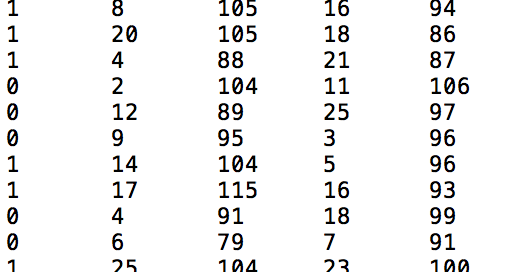
\includegraphics[width=8cm, height=4cm]{converted}
 \caption{converted data}
 \end{figure}
 \\
 After extracting the box scores, I did some data analysis for features.
 
 I first implemented the naive majority classifier based on the winning percentage of two teams in a game. 
\\
\\
\\
\\
\begin{center}
\begin{tabular}{|l|l|}
\hline
Params    & Meaning           \\ \hline
pr & Probability of winning \\ \hline
win-count & Times of winning \\ \hline
count & Total times of games of teams \\ \hline
predict-correct & Times of correct prediction  \\ \hline
total-instance & Number of instances \\ \hline
\end{tabular}
\end{center}
Each time I read one instance and predict the result based on winning probability of the visitor team and the home team. And I check whether the prediction is correct or not, if it's correct, I'll increase predict-correct and win-count of the visitor team by one, otherwise increase win-count of the home team by one and compute the pr for both teams. After all instances processed, I can get the ratio of predict-correct over total-instance to get the accuracy.
\\
\begin{center}
\begin{tabular}{|l|l|}
\hline
season    & accuracy           \\ \hline
2011-2012 & 0.6363636363636364 \\ \hline
2012-2013 & 0.6403580146460537 \\ \hline
2013-2014 & 0.6455284552845528 \\ \hline
2014-2015 & 0.647479674796748  \\ \hline
2015-2016 & 0.6304559270516718 \\ \hline
\end{tabular}
\end{center}
 This mechanism determines the winner by looking at whose current winning percentage is greater in this season. Of course at the beginning they may be both 0 as no matches between them, and in this case I'll random a real number between 0 to 1 and I predict team A is the winner if this number is less than 0.5. I tested it on dataset of 2013-2014, 2014-2015 and 2015-2016 and the accuracy is around 64\%. To deal with the data, I'm still using Java because I don't have too much experience with Matlab, which takes me more time. This is the first progress when comparing with other people's idea. After gathering behavior's data for both teams in each game, I'll use PCA(Principal  Component Analysis) to increase the convergence and reduce the dimension. When all feature vectors are ready, I'll go ahead to train the datasets with Linear Regression, Maximum Likelihood Classifier and SVM. Our goal is that the implemented algorithm should give better prediction result than the Naive majority classifier with around 64\%.
 
 For each group of features listed at the beginning of the Model section, I used them to make online predictions for the games and computed the accuracy based on the current value of features:
 \begin{figure}[htbp]
 \centering
 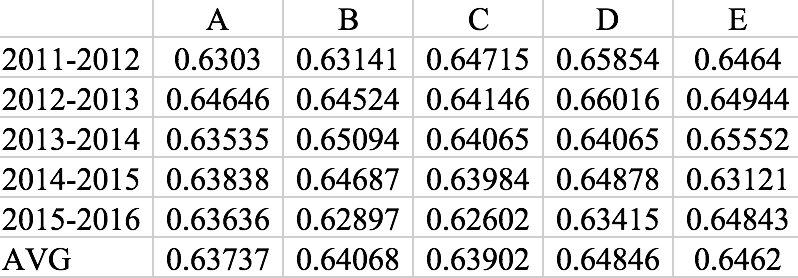
\includegraphics[width=8cm, height=4cm]{dataanalysis}
 \caption{The accuracy of prediction over all features}
\end{figure}
\\
We can see that the accuracy of prediction for 2015-2016 seasonal games is comparatively below the average. And that's because we only have 900 more games in this season while 1200 more in the others.

Also here I am taking $N$ equals to 10 because I did the following analysis:
 \begin{figure}[htbp]
 \centering
 \includegraphics[width=9cm, height=8cm]{bestN}
  \caption{The accuracy of prediction by win percentage with different N}
\end{figure}
\\
 As we can see in the figure, the accuracy climbs up quickly with the increasing number of recent games we are looking at. And it reaches the top when $N$ is equal to 10. After that, it starts to decrease. So here I decided to look at the recent 10 games for the win percentage. The same idea can be used for looking at the recent 11 games for the points differential after analysis.
 
 \section {Algorithm and Evaluation}
 \textbf{Support Vector Machine}
 \\
 \\
 To train and predict the result, what I'm using at first is SVM(Support Vector Machine), which constructs a hyperplane or set of hyperplanes in a high- or infinite-dimensional space. Since my data was stored into $Matlab$, and there're some existing calls about SVM, I decided to try SVM at first.
 \\
 I started with the function call $fitcsvm$ with linear kernel function to train a svm model from the training data. 
 After getting the model, I test it on the following year seasonal games, and found the accuracy is pretty good:
  \begin{figure}[htbp]
 \centering
 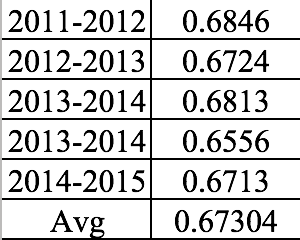
\includegraphics[width=4cm, height=2.5cm]{svmresult}
  \caption{SVM accuracy}
\end{figure}
\\
The running result of generating the prediction model is like:
 \begin{figure}[htbp]
 \centering
 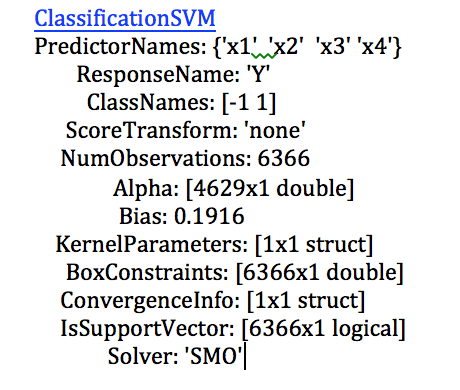
\includegraphics[width=6cm, height=5cm]{svm}
  \caption{SVM Model}
\end{figure}
\\
We can see that the SVM with linear kernel works pretty well for this model, so we can say that it's more likely that it's linear separable. If the accuracy is pretty low, then I'll assume that it may be not linear separable or there're lots of noise. And in that case, I may move on and try Gaussian Kernel or Polynomial kernel. Since it's more likely to be linear separable, I'll use linear regression in next section.
\\
\\
\textbf{Linear Regression}
\\
\\
The second method implemented is the linear regression. The method consists of multiplication of each feature by a weight, making a summation of all values obtained and a bias, and uses this final value for the classification:
\begin{equation}
Y = \omega_0+\sum_{i=1}^{n}{\omega_i*x_i}
\end{equation}
\\
I computed $Y$, and if $Y$ is greater than 0, the visitor team is considered the winner and otherwise the home team is considered the winner. 
\\
\\
The important part here is to determine the value of vector $w$. I tried to train on all feature vectors with stochastic gradient descent to obtain the convergence for $w$. However, I tried several settings of step size and iteration numbers, yet the experiment showed that even after 3*$10^{5}$ iterations some of variables still didn't converge.
\\
The figure below shows one of the variables:
\\
 \begin{figure}[htbp]
 \centering
 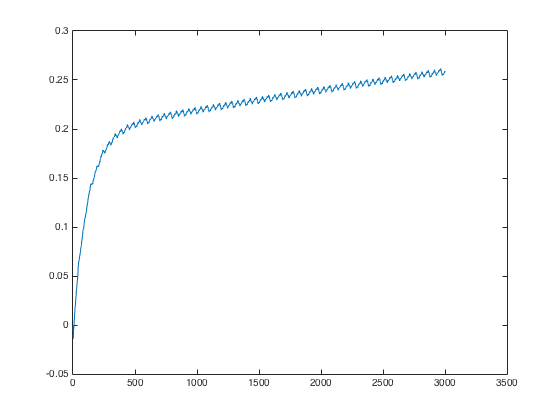
\includegraphics[width=9cm, height=6cm]{notconverge}
  \caption{Not converged}
\end{figure}
\\
So to boost the convergence, the method I used was to apply PCA(Principle Component Analysis). With PCA, we can decrease the number of features and thus the variables will be more likely to converge more quickly.
By loading feature vectors into $Matlab$, we can use predefined functions to compute the eigenvalues of covariance matrix:
 \begin{figure}[htbp]
 \centering
 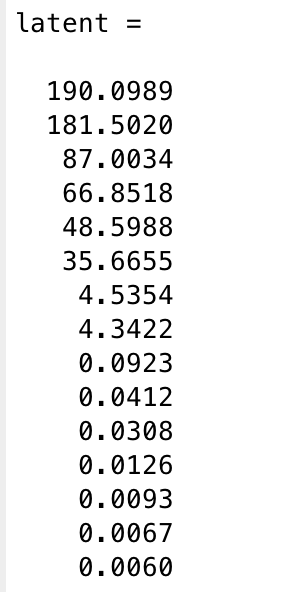
\includegraphics[width=3cm, height=8cm]{latent}
  \caption{Eigenvalues of covariance matrix}
\end{figure}
\\
And then the contribution percentage can be derived by the command $cumsum(latent)./sum(latent)$.
\\ 
Based on the contribution, we can set a threshold to 80\%. According to the figure below, we can say that the first four features can be used :
\\
\\
 \begin{figure}[htbp]
 \centering
 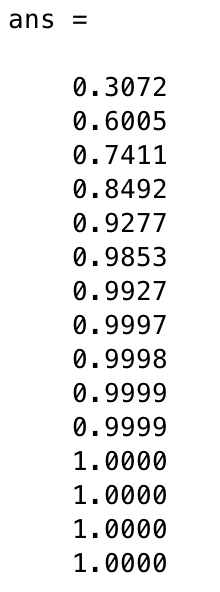
\includegraphics[width=3cm, height=8cm]{contribution}
  \caption{Eigenvalues of covariance matrix}
\end{figure}
\\
And the PCA feature vectors can be computed with the reduced features projected into the new space. Note that I preprocessed the value of features with -9999 as there's no data for each team at the beginning. So I removed the unpredicted instances which will make the training and learning process become more accurate and convincing. And the weight vectors can converge as shown:
\begin{figure}[htbp]
 \centering
 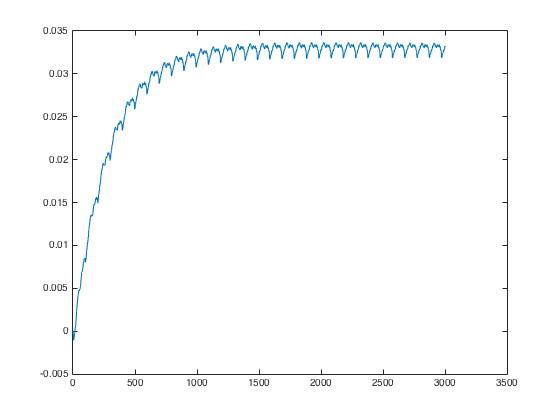
\includegraphics[width=8cm, height=6cm]{converged}
  \caption{Convergence of variables}
\end{figure}
\\
Weight vectors can be derived:
-0.0762    0.1008    0.0771    0.0027    0.0563
And the accuracy of prediction is shown as follows:
\begin{center}
\begin{tabular}{|l|l|}
\hline
season    & accuracy           \\ \hline
2011-2012 & 0.6789 \\ \hline
2012-2013 & 0.6942 \\ \hline
2013-2014 & 0.6391 \\ \hline
2014-2015 & 0.6718  \\ \hline
2015-2016 & 0.6522 \\ \hline
Avg & 0.66924 \\ \hline
\end{tabular}
\end{center}
From the result, we can see that the average accuracy of linear regression is approaching 67\%, which is higher than naive majority voting classifiers.
\\
\\
\\
\textbf{Multilayer Perceptron}
\\
\\
A multilayer perceptron (MLP) is a feedforward artificial neural network model that maps sets of input data onto a set of appropriate outputs. One characteristic of this algorithm is backpropagation. Here I used MLP for the prediction of the result of the game. 
The basic implementation is from Yu Hen Hu, and the mechanism involves randomly picking samples to train, feed-forwarding phase to compute sum of square errors, doing the error back-propagation phase to compute error and updating the weight matrix using gradient and some other parameters.

Each experiment will be executed for three loops and get the mean of the rate. The $\alpha$ vector is defined as [0.1 0.3 0.6 0.9] and $momentum$ is defined as [0.25 0.5 0.75]. With several configurations of different number of hidden layers, different number of neurons, the learning rate $\alpha$, and the value of momentum, the prediction rate can be obtained as follows:
\begin{figure}[htbp]
 \centering
 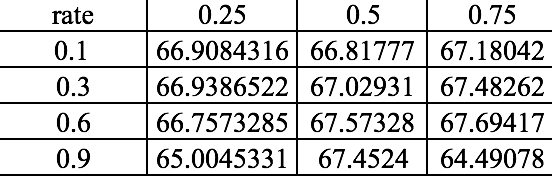
\includegraphics[width=7cm, height=2.5cm]{rate1}
  \caption{One hidden layer and four neurons}
\end{figure}
\begin{figure}[htbp]
 \centering
 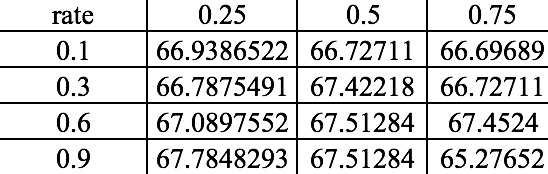
\includegraphics[width=7cm, height=2cm]{rate2}
  \caption{One hidden layer and eight neurons}
\end{figure}
\begin{figure}[htbp]
 \centering
 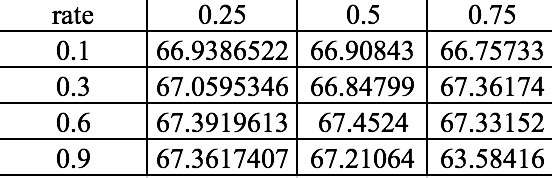
\includegraphics[width=7cm, height=2cm]{rate3}
  \caption{One hidden layer and twelve neurons}
\end{figure}
\\
We can observe that adding more neurons do increase the performance to some degree. Note that too few hidden units will generally leave high training and generalization errors due to under-fitting. Too many hidden units will result in low training errors, but will make the training unnecessarily slow, and will often result in poor generalization.
After training the data with one configuration, I test it on the test data and evaluate it. Each time I recorded the best accuracy and found one good model with the configuration of two hidden layers with eight and twelve neurons in each layer respectively. The accuracy on the models is computed:
\begin{center}
\begin{tabular}{|l|l|}
\hline
season    & accuracy           \\ \hline
2011-2012 & 0.6917 \\ \hline
2012-2013 & 0.6872 \\ \hline
2013-2014 & 0.6915 \\ \hline
2014-2015 & 0.6899  \\ \hline
2015-2016 & 0.6877 \\ \hline
Avg & 0.6896 \\ \hline
\end{tabular}
\end{center}

As we can see, multilayer perceptron algorithm works the best of the algorithms implemented with almost 69\%.

\section{Related work}
There's a project from \url{http://www.mbeckler.org/coursework/2008-2009/10701_report.pdf}  by Matthew and Michael. What they did was to use SQL to store all players' statistics to obtain the statistics of each team. And then they used algorithms for training and prediction with the assistance of K-means and Approximate Value. They did good job in prediction outcome of games with regards to the team's statistics. And their work can achieve about 73\% accuracy, which is really good because of solid data preparation. But my work is based on only the box scores, and I also takes the recent win percentage and point differentials into consideration to measure the recent performance of teams and I explore several algorithms for the best classification method.

\section {Conclusion, Limitations, and Future Work}
I collected box scores for each NBA seasonal game and converted to the dataset we need. And I  performed data analysis for the features I defined, also the accuracy of naive majority voting was computed as our initial goal. After that I implemented several algorithms, PCA was used to boost convergence in linear regression. For MLP, I tested many different configurations on the parameters.  And the result is that MLP is the best algorithm with around 69\% accuracy and both SVM and linear regression yield about 67\% accuracy. All of the implemented algorithm achieved the goal of 64\% by the naive majority voting mechanism. 
\\
\\
And the limitation of my work is that I don't import the statistics of players or teams. So in the future, I should follow Matthew and Michael's work to build SQL and grasp all player's performance to compute the statistics for all teams. With the comprehensive performance by analyzing the box scores and the the generated detailed teams' statistics, the prediction can be expected to be more accurate.
% In the unusual situation where you want a paper to appear in the
% references without citing it in the main text, use \nocite
\nocite{langley00}

\bibliography{example_paper}
\bibliographystyle{icml2016}

\end{document} 


% This document was modified from the file originally made available by
% Pat Langley and Andrea Danyluk for ICML-2K. This version was
% created by Lise Getoor and Tobias Scheffer, it was slightly modified  
% from the 2010 version by Thorsten Joachims & Johannes Fuernkranz, 
% slightly modified from the 2009 version by Kiri Wagstaff and 
% Sam Roweis's 2008 version, which is slightly modified from 
% Prasad Tadepalli's 2007 version which is a lightly 
% changed version of the previous year's version by Andrew Moore, 
% which was in turn edited from those of Kristian Kersting and 
% Codrina Lauth. Alex Smola contributed to the algorithmic style files.  
